\documentclass[uplatex,dvipdfmx]{bxjsarticle}

\usepackage{listings}
\usepackage{xcolor}
\usepackage{hyperref}
\usepackage{graphicx}
\usepackage{amsmath}
\usepackage{geometry}
\geometry{margin=25mm}

% Ciscoコマンド用の設定
\lstdefinelanguage{Cisco}{
  morekeywords={enable,configure,terminal,interface,router,network,ip,route,show,version,exit,no,auto-summary},
  sensitive=false,
  morecomment=[l]{!},
  morestring=[b]",
}

\lstset{
  language=Cisco,
  basicstyle=\ttfamily\small,
  keywordstyle=\color{blue}\bfseries,
  commentstyle=\color{gray},
  stringstyle=\color{orange},
  backgroundcolor=\color{gray!10},
  frame=single,
  breaklines=true,
  captionpos=b,
  numbers=left,
  numberstyle=\tiny\color{gray},
  xleftmargin=1.5em,
  xrightmargin=1.5em
}

\title{Ciscoルーター設定備忘録}
\author{Yuiki Nakanishi}
\date{\today}

\begin{document}

\maketitle

\section{ケーブルの種類}

同じ種類のケーブルを接続する場合はクロスケーブル,違う種類の場合はストレートケーブル.

\begin{figure}[htbp]
  \centering
  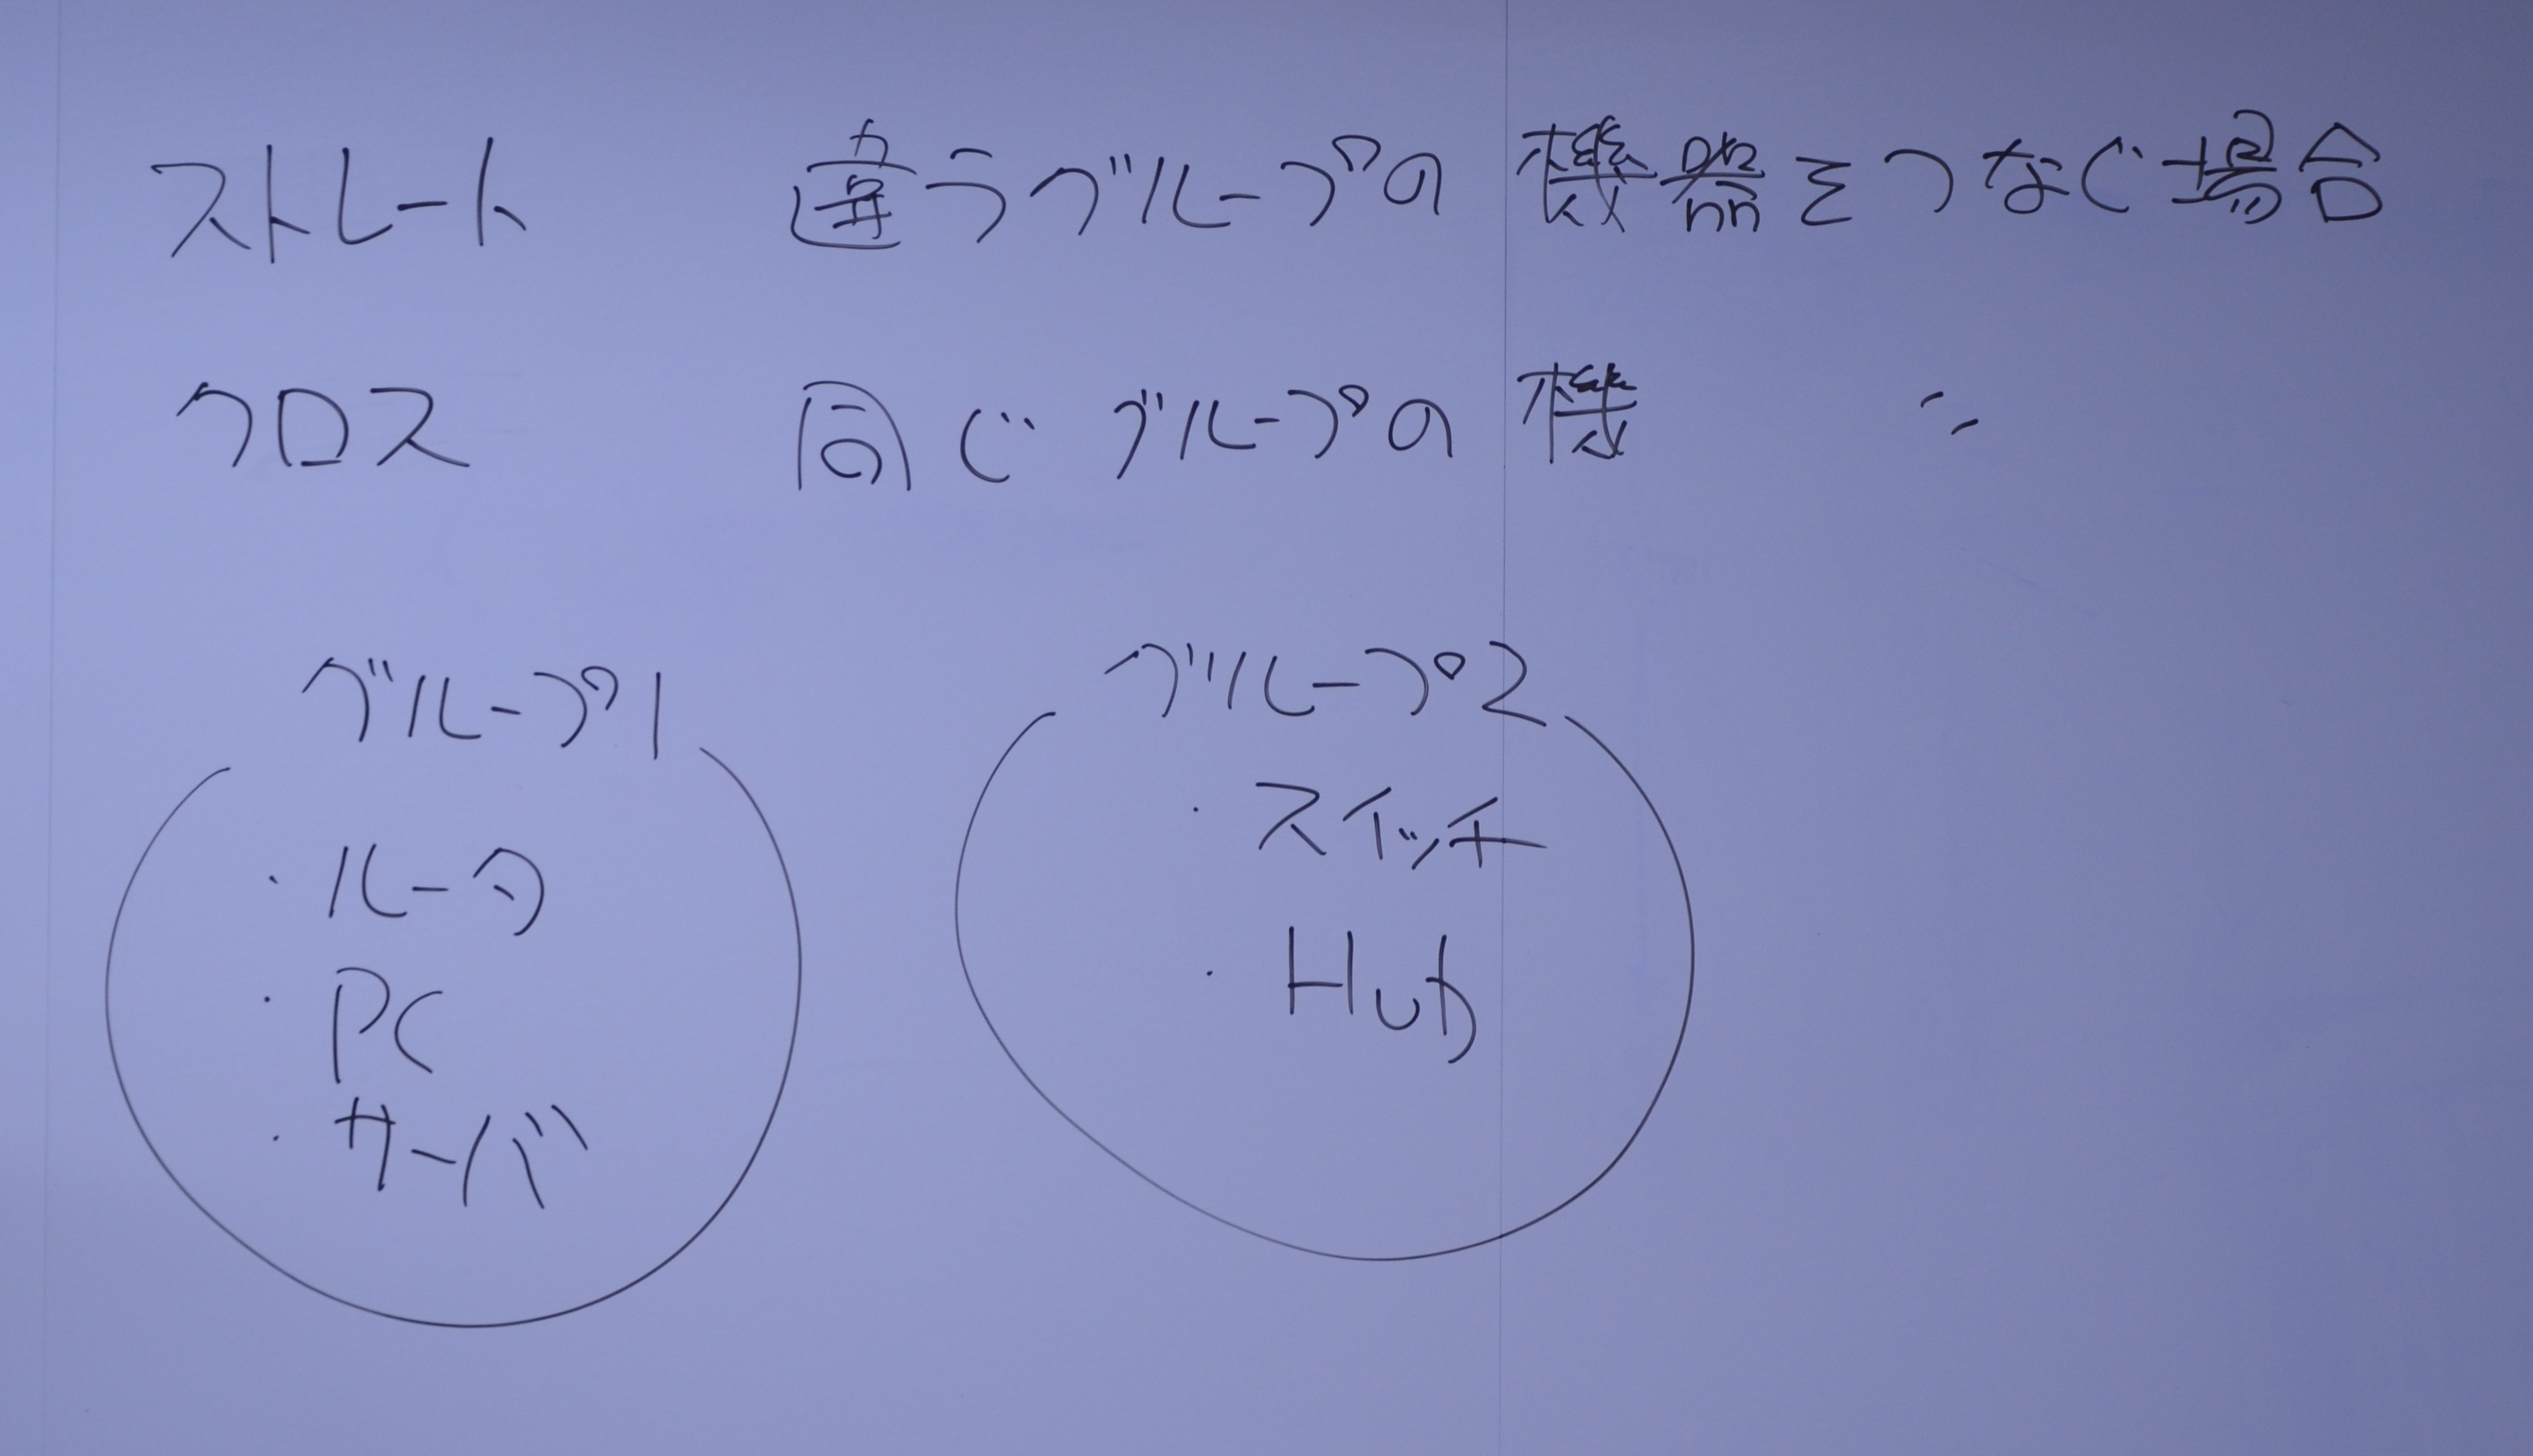
\includegraphics[width=1\linewidth]{figure/lan.JPG}
\end{figure}

\section{モードの移動}

\subsection{管理者になる}

\begin{lstlisting}[caption={管理者になる}]
> enable
\end{lstlisting}

\subsection{コンフィグモードに入る}

\begin{lstlisting}[caption={コンフィグモードに入る}]
# config terminal
\end{lstlisting}

\section{ホスト名の変更}

\begin{lstlisting}[caption={ホスト名の変更}]
(config) hostname XX  // hostname を XX に変更する.
\end{lstlisting}

\section{IP Address 設定}

\begin{lstlisting}[caption=IP Address Settings]
en
conf t
int fa ?/?  // LAN ポート番号
ip address 192.168.1.0  255.255.255.0 // IP Address,Subnet Mask
no shut
\end{lstlisting}

\section{設定の管理}

\subsection{設定の表示}

\begin{lstlisting}[caption={設定の表示}]
# show running-config
\end{lstlisting}

\subsection{保存されている設定の表示}

\begin{lstlisting}[caption={保存されている設定の表示}]
# show startup-config
\end{lstlisting}

\subsection{設定の保存}

\begin{lstlisting}[caption={設定の保存}]
# copy running-config startup-config
\end{lstlisting}

\section{パスワードの設定}

\subsection{管理者のパスワード}

\begin{lstlisting}[caption={管理者のパスワード}]
(config#) enable secret XXXX  // XXXX というパスワードを設定する.
\end{lstlisting}

\subsection{コンソールのパスワード}

\begin{lstlisting}[caption={コンソールのパスワード}]
(config)# line con 0
(config-line)# password XXXX
(config-line)# login
\end{lstlisting}

\subsection{TELNET のパスワード}

\begin{lstlisting}[caption={TELNET のパスワード}]
(config)# line vty 0 4
(config-line)# password XXXX
(config-line)# login
(config)# service password-encryption
\end{lstlisting}

\section{スタティックルートの設定}

\begin{lstlisting}[caption={スタティックルートの設定}]
(config)# ip route 宛先ネットワークアドレス 宛先サブネットマスク ネクストホップ
// 設定を削除する場合
(config)# no ip route xxx.xxx.xxx.xxx yyy.yyy.yyy.yyy zzz.zzz.zzz.zzz
\end{lstlisting}

\section{デフォルトルートの設定}

\begin{lstlisting}[caption={デフォルトルートの設定}]
(config)# ip route 0.0.0.0 0.0.0.0 <ネクストホップ>

\end{lstlisting}

\section{RIPの設定}

RIPの設定は以下の通りです。

\begin{lstlisting}[caption=RIP Settings]
router rip
network 192.168.1.0 // ルータにつながっている全ての IP Address を記述する.
\end{lstlisting}

設定中のコマンドは、例えば \texttt{router rip} や \texttt{no auto-summary} のように行中に記述できます。

\section{EIGRPの設定}

\begin{lstlisting}[caption=EIGRP Settings]
router eigrp 100
network 192.168.1.0 // ルータにつながっている全ての IP Address を記述する.
\end{lstlisting}

\section{Changing Administrative Distance}

ルーティングプロトコルの優先順位

\begin{lstlisting}[caption=Changing Administrative Distance]
router rip
distance 80 // 1 が最も優先順位が高い
\end{lstlisting}



\end{document}
